ในส่วนของงานวิจัยสิ่งที่เราให้ความสนใจ คือ ข้อมูลการกระทำของมนุษย์แต่ละคนภายในวิดีโอ  ซึ่งเพื่อที่เราจะได้ผลลัพธ์ที่มีประสิทธิภาพออกมาเป็นข้อมูลของสิ่งที่เราสนใจและสามารถนำไปใช้ต่อได้ เราจึงจำเป็นจะต้องใช้การวิเคราะห์ผลวิดีโอเพื่อที่จะสกัดสิ่งที่เราสนใจออกมาจากวิด๊โอ ซึ่งการวิเคราะห์ผลวิดีโอมีหลากหลายกระบวนการในการทำ จะทำทีละขั้นตอน โดยในแต่ละกระบวนการจะมีจุดประสงค์ของการทำและผลลัพธ์หลังการทำที่แตกต่างกัน ในหัวข้อนี้จะมาอธิบายถึงกระบวนการในการวิเคราะห์ผลของวิดิโอและผลลัพธ์ของการทำกระบวนการนั้น

\subsubsection*{2.1.1 การตรวจจับวัตถุ}
การตรวจจับวัตถุเป็นสิ่งที่สำคัญเป็นอันดับต้นๆของการวิเคราะห์ผลของวิดีโอ คือ การตรวจจับวัตถุ กล่าวคือกระบวนการที่ผู้วิจัยจะต้องทำคือระบุสิ่งที่สนใจว่าคืออะไร อยู่ตำแหน่งใด ซึ่งในปัจจุบันการทำการตรวจจับวัตถุมักนำ Machine learning model มาใช้เพื่อช่วยตรวจจับวัตถุที่เราสนใจ ซึ่ง Machine learning model ที่เราเลือกใช้คือ YOLO v3 โดยเหตุผลที่เราเลือกใช้ Machine learning model YOLO v3 จะถูกกล่าวไว้อยู่ในหัวข้อ Machine learning model ในหัวข้อถัดไป
\par
YOLO v3 เป็น Machine learning model ที่ในปัจจุบันนิยมนำมาใช้ตรวจจับวัตถุในงานวิเคราะห์ผลของวิดีโอ เนื่องจากสามารถตรวจจับวัตถุได้แบบเรียลไทม์และมีความแม่นยำ โดยหลักการของ YOLO v3 คือ นำรูปภาพที่ต้องการตรวจจับตำแหน่งของวัตถุผ่าน neural network โดยโครงข่ายจะแบ่งรูปภาพเป็นพื้นที่ และ จะทำนายกรอบสี่เหลี่ยมพร้อมกับทำนายความน่าจะเป็นของแต่ละหมวดหมู่ในแต่ละพื้นที่ สุดท้ายจะเลือกกรอบสี่เหลี่ยมและหมวดหมู่ที่มีค่าคะแนนความน่าจะเป็นมากที่สุด

\subsubsection*{2.1.2 การทำนายตำแหน่งถัดไปของวัตถุ (Tracking)}
การติดตามการเคลื่อนไหวของวัตถุ\textsuperscript{\cite{danelljan2014accurate}} คือระบบที่ใช้สำหรับการติดตามการเคลื่อนไหวของวัตถุที่สนใจที่อยู่ในรูปภาพ 
โดยใช้การคำนวณทางคณิตศาสตร์ และการประมวลผลภาพ (image processing) ทำให้การประมวลผลนั้นเร็วกว่าการใช้โมเดลปัญญาประดิษฐ์ ซึ่งอัลกอริทึมติดตามการเคลื่อนไหวที่นิยมใช้มีสองอัลกอริทึม
คือ correlation filter และ kalman filter ซึ่งหลักการของทั้งสองอัลกอริทึมนั้นจะแตกต่างกันโดยที่ correlation filter นั้นจะใช้พิกเซลของวัตถุในการคำนวณตำแหน่งถัดไปของวัตถุ 
และ kalman filter จะใช้ข้อมูลการเคลื่อนไหวในการคำนวณตำแหน่งถัดไปของวัตถุ ซึ่งจากการศึกษาในบทความ "Object Tracking using Correlation,
Kalman Filterand Fast Means Shift Algorithms"\textsuperscript{\cite{ali2006object}} kalman filter มีประสิทธิภาพที่สูงนั้นจะขึ้นอยู่กับข้อมูลที่ได้จากการวัด (measurement)
และความซับซ้อนในการเคลื่อนไหวของวัตถุ ในขณะที่ correlation นั้นมีประสิทธิภาพที่ด้อยกว่า kalman filter เพียงเล็กน้อยและสามารถติดตามการเคลื่อนไหวที่ซับซ้อนของวัตถุได้ดีกว่า 
(การเคลื่อนไหวที่ซับซ้อนหมายถึง การเคลื่อนไหวที่เกิดการเปลี่ยนทิศทางฉับพลันบ่อย) ผู้วิจัยจึงตัดสินใจเลือกใช้ correlation filter ในงานครั้งนี้
\begin{figure}[!ht]
	\centering
	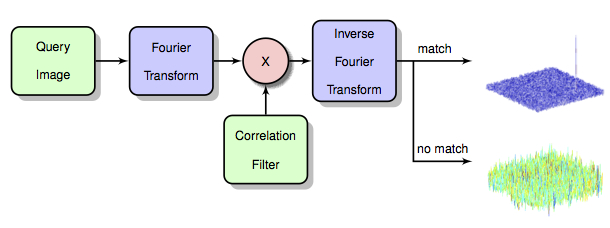
\includegraphics[width=1\textwidth]{chapter2/images/track-concept.png}
		\caption[แนวคิดของระบบติดตามการเคลื่อนไหวของวัตถุ]{แนวคิดของระบบติดตามการเคลื่อนไหวของวัตถุ\textsuperscript{\cite{correlation_filter}}}
    	\label{fig:Track_concept}
\end{figure}

จากรูปที่ \ref{fig:Track_concept} เป็นหลักการในการติดตามการเคลื่อนไหวของวัตถุแบบ correlation filter โดยการนำรูปมาผ่านกระบวนการแปลงฟูรีเยร์ (fourier transform)
และนำมาคูณกับ correlation filter ซึ่งเป็นตัวกรองที่ใช้สำหรับการหาความสัมพันธ์กับวัตถุในภาพ จากนั้นทำการแปลงฟูรีเยร์ผกผัน (inverse fourier transform) 
เพื่อตรวจสอบว่าวัตถุในภาพนั้นอยู่ที่ตำแหน่งใด โดยมีการคำนวณเริ่มจากการหา correlation filter ที่ดีที่สุดโดยใช้วิธีลดผลรวมของข้อผิดพลาดกำลังสองให้น้อยที่สุดดังนี้

\begin{equation}
\epsilon = \left \| \sum_{l = 1}^{d} h^{l} \star f^{l} - g \right \|^2 + \lambda \sum_{l = 1}^{d}\left \| h^{l} \right \|^2
\end{equation}
โดยที่
\begin{conditions}
 \epsilon     	&   ค่าความคลาดเคลื่อน 							\\
 d      		&  จำนวนมิติของผังคุณลักษณะของภาพ  \\   
 h 			&  correlation filter								\\
\star 			&  circular correlation							\\
 f			&  พื้นที่สี่เหลี่ยมของวัตถุที่สนใจที่ได้จากการทำผังคุณลักษณะ	\\
 g			&  ผลลัพธ์ correlation ที่ต้องการของ f					\\
 \lambda   		&  regularization term
\end{conditions}

เมื่อพิจารณาจากรูปภาพเดียวในกรณีที่เวลา ($t$) เท่ากับ 1 จะสามารถจัดรูปสมการด้านบนได้ดังนี้ 

\begin{equation}
H^{l} = \frac{\bar{G}F^{l}}{\sum_{k=1}^{d}\bar{F^{k}}F^{k} + \lambda}
\end{equation}
\begin{equation}
H_{t}^{l} = \frac{A_{t}^{l}}{B_{t}}					
\end{equation}					
\begin{equation}
A_{t}^{l} = (1-\eta )A_{t-1}^{l} + \eta \bar{G_{t}}F_{t}^{l}
\end{equation}
\begin{equation}
B_{t} = (1-\eta )B_{t-1} + \eta \sum_{k=1}^{d}\bar{F_{t}^{k}}F_{t}^{k}
\end{equation}
\clearpage
\noindent
โดยที่
\begin{conditions}
 H 		     	&   correlation filter								\\
 \eta      		&  อัตราการเรียนรู้						 		\\   
 \bar{G} 		&  g ที่ผ่านการทำ complex conjugation					\\
 F			&  พื้นที่สี่เหลี่ยมของวัตถุที่สนใจที่ได้จากการทำผังคุณลักษณะ	\\
 \bar{F}		&   f ที่ผ่านการทำ complex conjugation					\\
 t 	  		&  เวลา
\end{conditions}
จากสมการที่ได้มาจะสามารถทำให้หาตำแหน่งต่อไปของวัตถุที่สนใจได้ด้วยสมการต่อไปนี้
\begin{equation}
y = F^{-1}\left \{ \frac{\sum_{l = 1}^{d} \bar{A^{l}}Z^{l}}{B + \lambda} \right \}
\end{equation}
โดยที่
\begin{conditions}
 y 		     	&   correlation score										\\
 F^{-1}    		&  การแปลงฟูรีเยร์ผกผันแบบไม่ต่อเนื่อง (inverse discrete fourier transform)						\\   	
 \bar{A}^{l} 	&  $A^{l}$ ที่ผ่านการทำ complex conjugation				\\
 Z	 		&  พื้นที่สี่เหลี่ยมของวัตถุที่สนใจที่ได้จากการหาผังคุณลักษณะของภาพใหม่	
\end{conditions}
โดยค่าของ $y$ ที่ได้ออกมาจะทำให้รู้ถึงตำแหน่งของวัตถุที่สนใจได้ ณ ตำแหน่งที่ $y$ มีค่าสูงสุด

\subsubsection*{2.1.3 การระบุตัวตนของบุคคล (ReID)}
ระบบระบุตัวตนของบุคคล\textsuperscript{\cite{luo2019alignedreid++}}\textsuperscript{\cite{zhang2017alignedreid}} คือการระบุตัวตนของบุคคลภายในวิดีโอหรือระหว่างสองภาพ สามารถนำมาประยุกต์ใช้ในด้านของการรักษาความปลอดภัย 
หรือการตามหาบุคคล ซึ่งการระบุตัวตนของบุคคลนั้นเป็นปัญหาที่ท้าทาย เนื่องจากคุณลักษณะทั่วไปของบุคคลในภาพไม่เพียงพอต่อการระบุตัวตนภายในภาพว่าเป็นบุคคลคนเดียวกันได้ ซึ่งวิธีการที่ใช้ในการระบุตัวตนของบุคคลเรียกว่า 
Dynamically Matching Local Information (DMLI) ที่สามารถจัดแนวรายละเอียดข้อมูลของภาพและเพิ่มประสิทธิภาพให้สูงขึ้น 
ถึงแม้ว่า DMLI นั้นจะไม่ใช่วิธีการที่มีประสิทธิภาพสูงสุดแต่มีประสิทธิภาพใกล้เคียงกับโมเดลอื่นๆ แต่ผู้วิจัยสามารถนำวิธีนี้มาประยุกต์เข้ากับงานวิจัยครั้งนี้ได้สะดวกที่สุด จึงนำวิธีการนี้มาใช้สำหรับงานวิจัยครั้งนี้

\begin{figure}[!ht]
	\centering
	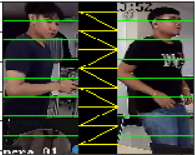
\includegraphics[width=0.3\textwidth]{chapter2/images/alignedreid.png}
		\caption{การแบ่งภาพออกเป็น 8 ส่วนของระบบระบุตัวตนของบุคคล}
    	\label{fig:alignedreid}
\end{figure}

การทำงานของระบบระบุตัวตนของบุคคลจะเริ่มจากการแบ่งภาพออกเป็น 8 ส่วนและนำคุณลักษณะทั่วไปของภาพมาผ่านกระบวนการ normalization เพื่อลดความซ้ำซ้อนของข้อมูล 
แล้วนำมาเปรียบเทียบความแตกต่างของคุณลักษณะทั่วไปของภาพโดยใช้วิธี euclidean distance หลังจากนั้นใช้วิธี DMLI หาความแตกต่างออกมา โดยค่าที่ได้ออกมาจะเรียกว่า aligned distance ถ้าค่าที่ออกมาใกล้เคียงกับศูนย์
จะหมายถึงบุคคลในภาพทั้งสองเป็นบุคคลเดียวกัน โดยใช้การกำหนดเกณฑ์ของ aligned distance สำหรับระบุตัวตนของบุคคลในภาพว่าเป็นบุคคลเดียวกันหรือไม่

โดยชุดข้อมูลที่นำมาใช้สำหรับการทำโมเดลปัญญาประดิษฐ์ได้แก่
\begin{enumerate}
	\item{Market1501 เป็นชุดข้อมูลที่เก็บข้อมูลภาพของบุคคลโดยใช้กล้องจำนวนหกตัว ถ่ายภาพบุคคลที่ด้านหน้าของซุปเปอร์มาร์เก็ตในมหาวิทยาลัย Tsinghua}
	\item{DukeMTMCReID เป็นชุดข้อมูลที่เก็บข้อมูลภาพของบุคคลโดยใช้กล้องจำนวนแปดตัว ถ่ายภาพบุคคลที่วิทยาเขตของมหาวิทยาลัย Duke ซึ่งมีการเก็บภาพมากถึงสองล้านภาพของนักศึกษาสองพันคน }
	\item{CUHK-03 เป็นชุดข้อมูลที่เก็บภาพของบุคคลที่มหาวิทยาลัยที่ฮ่องกง}
	\item{MSMT17 เป็นชุดข้อมูลที่เก็บข้อมูลภาพของบุคคลโดยใช้กล้องจำนวนสิบห้าตัว โดยที่กล้องแต่ละตัวจะไม่ได้ตั้งอยู่สถานที่เดียวกัน และเก็บข้อมูลที่ในวันที่มีสภาพอากาศต่างกัน}
\end{enumerate}

โดยทุกชุดข้อมูลจะใช้โครงสร้าง (architecture) ResNet50 ในการสร้างโมเดลปัญญาประดิษฐ์ และทดสอบด้วยวิธี Global+DMLI คือการนำคุณลักษณะทั่วไปและคุณลักษณะจำเพาะของภาพที่ได้มาจากโมเดลปัญญาประดิษฐ์ นำมาหาค่าระยะความแตกต่าง โดยที่ค่าระยะความแตกต่างของคุณลักษณะทั่วไปสามาหาได้โดยใช้วิธี Euclidean distance และค่าระยะความแตกต่างของคุณลักษณะจำเพาะสามารถหาได้โดยใช้วิธี DMLI และนำมาเทียบกับชุดข้อมูลทดสอบเพื่อคำนวณหาค่า rank1 และ mAP โดยที่ค่า rank1 หมายถึงค่าอัตราร้อยละของความมั่นใจสูงสุดของโมเดลปัญญาประดิษฐ์ที่ทำนายออกมาถูกต้อง 
และค่า mAP คือการหาค่าเฉลี่ยความแม่นยำในแต่ละหมวดหมู่ ซึ่งสามารถดูค่า rank1 และ mAP ของโมเดลปัญญาประดิษฐ์สำหรับการทำระบุตัวตนของบุคคลได้ในหัวข้อที่ \ref{sec:reid_ex}

วิธีการคำนวณของ DMLI ในขั้นตอนการสร้างโมเดลปัญญาประดิษฐ์ของการระบุตัวตนบุคคล
\begin{equation}
d_{i,j} = \frac{e^{\left \| f_{i} - g_{j} \right \|^{2}} - 1}{e^{\left \| f_{i} - g_{j} \right \|^{2}} + 1} \qquad i,j \epsilon 1,2,3,..H
\end{equation}

โดยที่
\begin{conditions}
d		&		เมทริกซ์ของระยะความแตกต่างที่น้อยที่สุดของคุณลักษณะจำเพาะของทั้งสองภาพ			\\
f		&		ค่าคุณลักษณะจำเพาะของรูปภาพที่ 1				\\
g		&		ค่าคุณลักษณะจำเพาะของรูปภาพที่ 2				\\
H		&		จำนวนภาพแนวตั่งที่แบ่งออกมา
\end{conditions}

\begin{equation}
S_{i,j} = \begin{cases}
d_{i,j} & \text{ if } i=1,j=1 \\ 
S_{i-1,j}+d_{i,j} & \text{ if } i\neq 1,j=1 \\ 
S_{i,j-1}+d_{i,j} & \text{ if } i=1,j\neq1 \\ 
min(S_{i-1,j},S_{i,j-1}) & \text{ if } i\neq1,j\neq1 
\end{cases}
\end{equation}

เมื่อทำการคำนวณ $S_{i,j}$ ซึ่งเป็นผลรวมของระยะความแตกต่างที่น้อยที่สุดแล้วตัวสุดท้ายของ $S_{i,j}$ จะเป็นระยะความแตกต่างที่น้อยที่สุดที่ของคุณลักษณะจำเพาะของทั้งสองภาพ แต่ในกรณีที่ทางผู้วิจัยนำมาใช้งานค่า $d_{i,j}$ นั้นจะเป็นค่าที่ได้มาจากการทำ euclidean distance แทน


\subsubsection*{2.1.4 การจดจำการกระทำ}
input{chapter2/action_label}